% Introdu��o
\chapter{Introduction}


% TODO: Add more references
% TODO: Add Google Trend Big Data image

In the last ten years, the search for terms such as big data, data analysis, and data visualization has increased enormously. There is a lot of reasons for this phenomenon, one of them is that with the computing power advancement we now have to deal with huge masses of data, which grows daily, from different sources in several formats in an incredibly short time. Therefore new challenges are rising in the data analysis field: How to process these immense quantities quickly and efficiently? How to visualize this amount of data? How to clean the dataset without losing important points?

When it comes to the data analysis field and the analyst is working with large datasets, is very common to have a lot of points with attributes very distant from the rest of the dataset. This happens because when more huge is your dataset, more easily you can find abnormal points that will be more distant from the normal distribution. This kind of behavior is important to the analyst study and discover more information about the dataset itself and with this, he could take more accurate decisions and propose better statements. Usually, this concern about anomalous data was not too relevant for the most researches, but this behavior is changing since significant information can be discovered analyzing those uncommon points.

These specific data with those characteristics is called \textit{Outliers} and is very decisive that the current data analysts pay more attention to those data, because important information may be hidden inside these peculiar data. For example, if we get an isolated dataset about NYC taxis from 2011 and analyze the frequency of requests at the entire year, it will appear a lot of points very distant from the average curve and this will indicate an unusual behavior in this collection.

Generally, the first step to take in this situation is to remove the irregular points and continue the processing with the rest of the dataset, but if we get another isolated dataset about the wind speed from the same NYC region and compare this exactly space of time, we will perceive few peaks of high speed indicating hurricane at the same time \cite{DBLP:journals/debu/FreireCVZ16} as presented in Figure \ref{fig:freire-paper-taxy-wind}. Analyses like this prove the importance of detect, study and interpret those outliers to increase the knowledge obtained from this dataset.

\begin{figure*}[t]
	\centering
	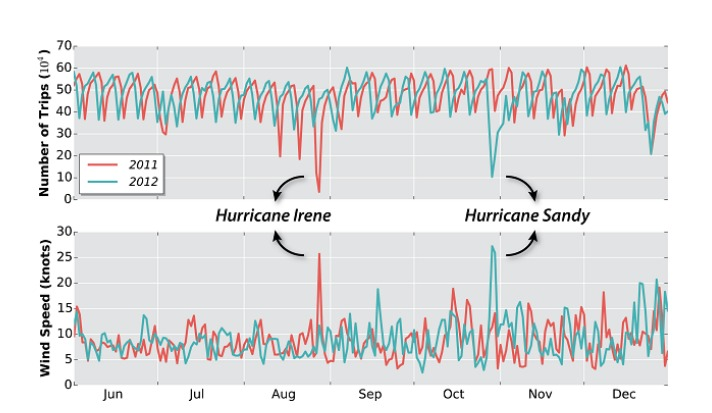
\includegraphics[width=\textwidth]{images/outlier-freire-figure-1}
	\caption{Figure taken from \cite{DBLP:journals/debu/FreireCVZ16} showing  relationship between the number of taxi trips over time and wind speed}
	\label{fig:freire-paper-taxy-wind}
	\vspace{-10pt}
\end{figure*}

\section{Context}

Nowadays we are more and more connected with multiple applications that access a huge
amount of our existing data and even generate more to improve their analyses about
us for diverses proposals. Tools like Google Maps, Uber, Waze has a lot of realtime
spatial data about our traffic behavior (private cars, public transportation, taxis,
etc.), work place, travel location, etc.

When it comes to regular users, it is very common that he will be lost in such masses
of spatial data and this will damage your possible analyse, even the simplest one.
This commom problem still does not have an definitively solution, so existing researches
trying to indicate possible approaches for mitigate this problem and be close to a
working solution. These approaches are based on: agroup a large amount of data by specific
attributes and summarize the commom attributes between those data for give simple
insights about these groups, filter the dataset to reduce the showing possibilities and
focus on specific data for a more detailed (but not wide) analysis, and a lot of others
strategies to reduce the complexity of the analysis.

Together with those most commom problems, exists an important one that can happen before
the first step of analysis that is: What do when parts of the dataset seems to be irregular
or with corrupted data? There are techniques that helps to clean those parts and not compromise
the analysis,
% citar algum artigo sobre limpeza de dados
but recently studies points the importance of these \textit{"abnormal"} data and how much
the analyst can learn just studying more precisely this set. \cite{DBLP:journals/debu/FreireCVZ16}

In this complex environment of spatial data analyses with a lot of variables and possibilities,
an user can easily fail in some of these step compromising severely the results of his analysis.
Combining all these details, we suggest an approach that take as relevant the user feedback
(capturing the mouse track) and based on those feedback, we will be able to analyse the user
interest and inside this we can detect, study and propose actions to perform when an data considered
outlier appears in this region of user interest.

\section{Objectives}

In this section are defined the general and specific objectives of the work.

\subsection{General Objectives}

\begin{itemize}
	\item
	      Introduce the problem of data analysis and visualization in large spatiotemporal
	      datasets nowadays.
	\item
	      Explain our proposed approach to detect spatial outliers in large datasets using
	      the concept of IDR and capturing user's feedback.
	\item
	      Present our results using the given approach to detect outliers in our spatial-temporal
	      environment and the benefits of these experiments.

\end{itemize}

\subsection{Specific Objectives}

\begin{itemize}
	\item
	      Analyze the latest researches in the field of outlier detection in spatial-temporal
	      datasets.
	\item
	      Present our proposed tool for spatial-temporal data analysis and visualization.
	\item
	      Compare the presented researches showing the pros and cons of each work.
	\item
	      Describe the concept of IDR used in our tool to mapping the user preference in a
	      spatial-temporal environment.
	\item
	      Summarize the most known existing outlier detection algorithms for generic and spatial
	      data.
	\item
	      Display our chosen outlier detection algorithm and explain the reasons for this choice.
	\item
	      Apply our IDR concept and our chosen outlier detection algorithm in a spatial-temporal
	      data environment.
	\item
	      Present the results of our application and indicate our future work.

\end{itemize}

\section{Work Organization}

The document is organized as follows. Section 2 summaries the existing researches
in data analysis and visualization field comparing with our proposed tool. Section 3 describes
the concepts of IDRs (Interesting Dense Region) and Outliers with the existing algorithms for
their detection and our chosen algorithm to detect outliers in our platform. Section 4 explains
how we apply the IDRs and outliers detection in the GeoGuide tool. Section 5 presents two
applications using distinct datasets to demonstrate the applicability of it to real-world
problems and the advantages of this approach. It shows and discusses the outlier detection
results. Finally, a conclusion and some directions for future works are given in Section 6.
